\chapter{Stand der Forschung} \label{ch:StandDerForschung}

Es soll ein Einblick auf den grundlegenden Hintergrund dieser Arbeit gegeben werden.
Deshalb wird in \secref{sec:TautochronerEntwurfAllgemein} die in \cite{Mayet:Tautochronic} entwickelte Formulierung
für den tautochronen Absorberentwurf dargelegt. 
Die Veranschaulichung der Sachverhalte, welche für diese Arbeit
grundlegend sind, steht dabei im Vordergrund.
Anschließend wird in \secref{sec:TheorieMistuning} der in \cite{Mayet:CPVAMitMistuning} vorgeschlagene
Mistuning-Ansatz eingeführt. Dabei werden die Auswirkungen des nichtlinearen
Mistuning-Ansatzes auf den zuvor in \secref{sec:TautochronerEntwurfAllgemein} skizzierten Formalismus aufgezeigt.


\section{Tautochroner Entwurf von Fliehkraftpendeln } 

\label{sec:TautochronerEntwurfAllgemein}


Die in diesem Abschnitt dargelegten Zusammenhänge stammen aus dem 
kürzlich veröffentlichten Paper \cite{Mayet:Tautochronic}.
Es werden die Sachverhalte veranschaulicht, welche für diese Arbeit
grundlegend sind und auf welchen im weiteren Verlauf aufgebaut wird bzw.
worauf sich an späterer Stelle wieder bezogen wird.
Dabei wird ein Einblick auf den grundlegenden Hintergrund dieser Arbeit gegeben,
ohne jedoch sämtliche Herleitungen und detaillierte Informationen wiederzugeben.
Für eine ausführliche und vollständige Darstellung sei an dieser Stelle
auf  \cite{Mayet:Tautochronic} verwiesen.


% Referenzen auf Gleichungen einfügen









\subsection[Systembeschreibung]{Systembeschreibung\footnote{Kapitel 3 in \cite{Mayet:Tautochronic}}}


\label{subsec:Systembeschreibung}



%%%%%%%%%%%%%%%%%%%%%%%%%%%%%%%%%%%%%%%%%%%%%%%%%%%%%%%%%%%%%%%%%%%%%%%%%%%%%%%%%%
% Ursprüngliche, viel ausführlichere Version
%%%%%%%%%%%%%%%%%%%%%%%%%%%%%%%%%%%%%%%%%%%%%%%%%%%%%%%%%%%%%%%%%%%%%%%%%%%%%%%%%%
%\subsubsection{Kinetische Energie}

Das in	\figref{fig:Theorie:BildCPVA} dargestellte Fliehkraftpendel
wird als Basis für die mathematische Beschreibung des mechanischen Systems
verwendet \cite{Mayet:Tautochronic}. Details zu diesem Fliehkraftpendeltyp sind
in \cite{mayet2012euromech} und Informationen zu damit durchgeführten, experimentellen Untersuchungen 
in \cite{Mayet:Experimental} zu finden.
%
%
\begin{figure}[ht]%
	\centering
			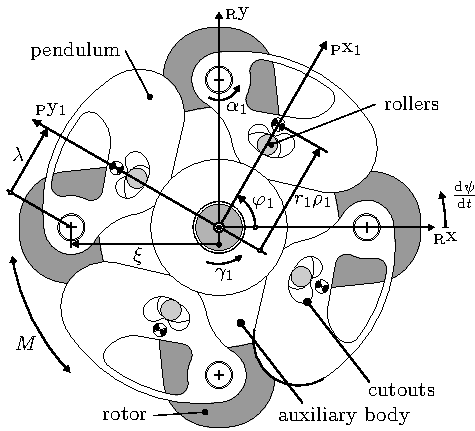
\includegraphics{PIC_120209_schematic_scpa_make}
			\caption[Schematische Darstellung eines Fliehkraftpendels]{Schematische Darstellung eines Fliehkraftpendels \cite{mayet2012euromech}}
	\label{fig:Theorie:BildCPVA}
\end{figure}
%
%
%
Der Rotor mit Freiheitsgrad $\psi(t)$ besitzt das Massenträgheitsmoment $\Theta_{Rotor}$.
Das dargestellte Absorbersystem besteht aus $n_p=4$ Pendeln, aus einem Hilfskörper ($n_a=1$)
und zugehörigen Wälzkörpern. 
Durch die kinematische Kopplung der vier Pendel über Hilfs- und Wälzkörper besitzt
das Fliehkraftpendelsystem nur einen Freiheitsgrad, welcher durch die generalisierte Koordinate $s(t)$
beschrieben wird. 
%
Jedes Pendel (Masse $m_i$, Massenträgheitsmoment $\Theta_{S,i}$ bezüglich seines Schwerpunkts und
Abstand $r_i \rho_i$ vom Drehpunkt des Rotors) kann Rotationen $\alpha_i(s)$ relativ
zum rotorfesten Koordinatensystem  $(\rs{_R}{x},\rs{_R}{y},\rs{_R}{z})$ ausführen. 
Die relative Rotation des Hilfskörpers (Massenträgheitsmoment $\Theta_{A,1}$ bezüglich seines Schwerpunkts)
wird mit $\gamma_1(s)$ bezeichnet und der Schwerpunkt des Hilfskörpers befindet sich in seinem
Drehpunkt. Dieser fällt mit dem Rotordrehpunkt zusammen, weshalb der Hilfskörper nur rotatorische
Bewegungen ausführen kann. Im allgemeinen Fall können beliebig viele Hilfskörper $n_a$ verwendet werden.
%
Der Winkel $\varphi_i (s)$ ist der Winkel zwischen dem rotorfesten Koordinatensystem 
$(\rs{_R}{x},\rs{_R}{y},\rs{_R}{z})$ und dem Koordinatensystem $(\rs{_P}[_i]{x},\rs{_P}[_i]{y},\rs{_P}[_i]{z})$, 
wobei der Schwerpunkt des $i$-ten Pendels auf der $\rs{_P}[_i]{x}$-Achse liegt.
%
Durch die Kontur der Ausfräsungen im Pendel und im Hilfskörper  können 
durch die kinematische Kopplung über die Wälzkörper beliebige,
nichtlineare, kinematische Zusammenhänge zwischen $\alpha_i(s)$ und $\gamma_1(s)$ vorgegeben werden.



Die Zeit $t$ wird in den folgenden Ausführungen mit der Mitteldrehzahl $\Omega$ des Rotors
skaliert und der Einfluss der Dynamik der Wälzkörper vernachlässigt.
Die skalierte Zeit wird mit $\tau = \Omega t$ bezeichnet und für Ableitungen 
nach $\tau$ wird die Abkürzung $ \dot{\left(\bullet\right)} =\frac{\dd}{\dd{\tau}}\left(\bullet\right)$ verwendet.

Die gesamte kinetische Energie $T_{tot}$ des Systems setzt sich aus den kinetischen Energien der einzelnen Körper zusammen
und ergibt sich zu
%
% Gesamte kinetische Energie
%
\begin{equation}
	T_{tot} = T_R + \sum_{i=1}^{n_p} T_{P,i} + \sum_{j=1}^{n_a} T_{A,j},
\label{eq:GesamteKinetischeEnergieTtot}
\end{equation}
%
%
%
wobei $T_R = \frac{1}{2}\Theta_{Rotor} \Omega^2 \dot{\psi}^2$ die kinetische Energie des Rotors, 
$T_{P,i}$ die kinetische Energie des $i$-ten Pendels 
\begin{equation}
	T_{P,i} = \frac{1}{2} m_i r_i^2 \left( \left(\pdiff{\rho_i}{s}\right)^2 \dot{s}^2 + \rho_i^2 \left(\pdiff{\varphi_i}{s}\dot{s}+\dot{\psi}\right)^2 \right) \Omega^2 
						+ \frac{1}{2} \Theta_{S,i} \left( \pdiff{\alpha_i}{s}\dot{s} + \dot{\psi} \right)^2 \Omega^2
\label{eq:KinetischeEnergiePendel}
\end{equation}
und $T_{A,j}$ die kinetische Energie des $j$-ten Hilfskörpers 
\begin{equation}
	T_{A,j} = \frac{1}{2} \Theta_{A,j} \left( \pdiff{\gamma_j}{s}\dot{s} + \dot{\psi} \right)^2 \Omega^2
\label{eq:KinetischeEnergieAuxiliaryBody}
\end{equation}
bezeichnet. $\rho_i (s)$ mit $\rho_i (0) = 1$ stellt den skalierten Abstand des $i$-ten Pendelschwerpunkts 
vom Rotordrehpunkt in Richtung der $\rs{_P}[_i]{x}$-Achse dar.
%
%
%
%
%%%%%%%%%%%%%%%%%%%%%%%%%%%%%%%%%%%%%%%%%%%%%%%%%%%%%%%%%%%%%%%%%%%%%%%%%%%%%%%%%%
%%%%%%%%%%%%%%%%%%%%%%%%%%%%%%%%%%%%%%%%%%%%%%%%%%%%%%%%%%%%%%%%%%%%%%%%%%%%%%%%%%
% Ursprüngliche, viel ausführlichere Version
%%%%%%%%%%%%%%%%%%%%%%%%%%%%%%%%%%%%%%%%%%%%%%%%%%%%%%%%%%%%%%%%%%%%%%%%%%%%%%%%%%
%%%%%%%%%%%%%%%%%%%%%%%%%%%%%%%%%%%%%%%%%%%%%%%%%%%%%%%%%%%%%%%%%%%%%%%%%%%%%%%%%%
%
% Kinetische Energie eines Hilfskörpers
%
%Der Hilfskörper $j$ mit Massenträgheitsmoment $\Theta_{A,j}$ kann nur rein rotatorische Bewegungen ausführen, weshalb sich dessen kinetische Energie zum einen aus dem Anteil der Rotation des rotorfesten Koordinatensystems $(\rs{_R}{x},\rs{_R}{y},\rs{_R}{z})$ und zum anderen aus dem Anteil der Drehung des Hilfskörpers $j$ um den Winkel $\gamma_j$ relativ zum rotorfesten Koordinatensystem zusammensetzt. 
%Die kinetische Energie $T_{A,j}$ des $j$-ten Hilfskörpers lautet
%\begin{equation}
%	T_{A,j} = \frac{1}{2} \Theta_{A,j} \left( \pdiff{\gamma_j}{s}\dot{s} + \dot{\psi} \right)^2 \Omega^2.
%\label{eq:KinetischeEnergieAuxiliaryBody}
%\end{equation}
%
%
% Kinetische Energie eines Pendels
%
%Die kinetische Energie des $i$-ten Pendels setzt sich sowohl aus translatorischen als auch aus rotatorischen Anteilen zusammen und kann unter Verwendung der bisher eingeführten Größen als
%\begin{equation}
%	T_{P,i} = \frac{1}{2} m_i r_i^2 \left( \left(\pdiff{\rho_i}{s}\right)^2 \dot{s}^2 + \rho_i^2 \left(\pdiff{\varphi_i}{s}\dot{s}+\dot{\psi}\right)^2 \right) \Omega^2 + \frac{1}{2} \Theta_{S,i} \left( \pdiff{\alpha_i}{s}\dot{s} + \dot{\psi} \right)^2 \Omega^2
%\label{eq:KinetischeEnergiePendel}
%\end{equation}
%geschrieben werden, wobei $\rho_i (s)$ mit $\rho_i (0) = 1$ den skalierten Abstand in Richtung der $\rs{_P}[_i]{x}$-Achse darstellt. Der Winkel $\varphi_i\left(s\right)$ ist der Winkel zwischen dem rotorfesten Koordinatensystem $(\rs{_R}{x},\rs{_R}{y},\rs{_R}{z})$ und dem Koordinatensystem $(\rs{_P}[_i]{x},\rs{_P}[_i]{y},\rs{_P}[_i]{z})$, wobei der Schwerpunkt des $i$-ten Pendels auf der $\rs{_P}[_i]{x}$-Achse liegt.
%
%
%%%%%%%%%%%%%%%%%%%%%%%%%%%%%%%%%%%%%%%%%%%%%%%%%%%%%%%%%%%%%%%%%%%%%%%%%%%%%%%%%%
%%%%%%%%%%%%%%%%%%%%%%%%%%%%%%%%%%%%%%%%%%%%%%%%%%%%%%%%%%%%%%%%%%%%%%%%%%%%%%%%%%
%
%
%
%
%
% Potential
%
Durch die spezielle Anwendung der Fliehkraftpendel zur Schwingungsreduktion bei Viertaktmotoren, bei welchen 
sich der Zylinderzyklus alle zwei Umdrehungen wiederholt, kann das anregende, externe Moment in Abhängigkeit
des Rotorwinkels $\psi$ geschrieben werden. Die potentielle Energie $V = V(\psi)$ lautet dann
\begin{equation}
		V\left(\psi\right) = - \int^{\psi}_{0} {M\left(\bar{\psi}\right) \dd \bar{\psi}} = M_0 \sin \left(k_E \psi\right) ,
\label{eq:PotentialDesAnregendenMoments}
\end{equation}
wobei das anregende Moment $M\left(\psi\right) = -k_E M_0 \cos \left(k_E \psi\right)$, welches auf den Rotor wirkt, 
als harmonische Anregung der Ordnung $k_E$ mit Amplitude $M_0$ angenommen wird (vgl. \secref{sec:Einl:Motivation}).
%
%
Für die Lagrange-Funktion $L = T_{tot} - V$ des betrachteten Systems resultiert dann
\begin{equation}
\begin{split} 
	L & = T_{tot} - V = T_R  + \sum_{j=1}^{n_a} T_{A,j} - V  + \sum_{i=1}^{n_p} T_{P,i} \\
		& = \frac{1}{2}\Theta_{Rotor} \Omega^2 \dot{\psi}^2 + \sum_{j=1}^{n_a} \left[\frac{1}{2} \Theta_{A,j} \left( \pdiff{\gamma_j}{s}\dot{s} + \dot{\psi} \right)^2 \Omega^2\right] - M_0 \sin \left(k_E \psi\right) \\
		& + \sum_{i=1}^{n_p} \left[\frac{1}{2} m_i r_i^2 \left( \left(\pdiff{\rho_i}{s}\right)^2 \dot{s}^2 + \rho_i^2 \left(\pdiff{\varphi_i}{s}\dot{s}+\dot{\psi}\right)^2 \right) \Omega^2 + \frac{1}{2} \Theta_{S,i} \left( \pdiff{\alpha_i}{s}\dot{s} + \dot{\psi} \right)^2 \Omega^2\right].   \end{split}
	\label{eq:LagrangeFunktionInRealenKoordinaten}
\end{equation}
%
%
%
%
%
%
%
%
%
%
%
%
%
%
%
%
%
%
%
%
%
%
%
%
%
%
%
%
%
%
%
%
%
%
%
%%%%%%%%%%%%%%%%%%%%%%%%%%%%%%%%%%%%%%%%%%%%%%%%%%%%%%%%%%%%%%%%%%%%%%%%%%%%%%%%%%
% Ursprüngliche, viel ausführlichere Version
%%%%%%%%%%%%%%%%%%%%%%%%%%%%%%%%%%%%%%%%%%%%%%%%%%%%%%%%%%%%%%%%%%%%%%%%%%%%%%%%%%
%\subsubsection{Skalierte Lagrange-Funktion}
%
Um  eine dimensionslose Darstellung für die einheitliche Systembetrachtung zu erhalten, wird Gleichung
\eqref{eq:LagrangeFunktionInRealenKoordinaten} mit $1/({\Theta_{Scale}\Omega^2})$ 
durchmultipliziert.
Dies führt nach  \cite{Mayet:Tautochronic} auf die \new{skalierte Lagrange-Funktion} 
$\tilde{L} = (T_{tot} - V)/(\Theta_{Scale}\Omega^2)$, welche als
%
\begin{equation}
\begin{split}  
	\tilde{L} &= \frac{1}{2} \epsilon^{-1} \dot{\psi}^2 + \frac{1}{2} \sum_{i=1}^{n_p} \left( \mu_{m,i}  \left( \left( \pdiff{\rho_i}{s} \right)^2 \dot{s}^2 + \rho_i^2 \left( \pdiff{\varphi_i}{s} \dot{s} 
																																											+ \dot{\psi} \right)^2 \right) + \mu_{r,i} \left( \pdiff{\alpha_i}{s} \dot{s} + \dot{\psi} \right)^2 \right) \\
						&+ \frac{1}{2} \sum_{i=1}^{n_a} \nu_j \left( \pdiff{\gamma_j}{s} \dot{s} + \dot{\psi} \right)^2  - \Gamma \sin\left( k_E \psi \right) \end{split}
\label{eq:SkalierteLagrangeFunktionfuereinAbsorbersystem}
\end{equation}
%
mit den abkürzenden Schreibweisen
%
\begin{equation}
\begin{split} 	\Theta_{Scale}&= \max \left( m_1 r_1^2, m_2 r_2^2, \dots, m_{n_p} r_{n_p}^2 \right),&		\Gamma&= \frac{M_0}{\Theta_{Scale} \Omega^2},& 			\nu_j&= \frac{\Theta_{A,j}}{\Theta_{Scale}},\\ 
								\mu_{m,i}&= \frac{m_i r_i^2}{\Theta_{Scale}},& 																					\mu_{r,i}&= \frac{\Theta_{S,i}}{\Theta_{Scale}},& 	\epsilon&= \frac{\Theta_{Scale}}{\Theta_{Rotor}} \end{split}
\label{eq:SkalierteLagrangeFunktionAbkuerzungen}
\end{equation}
%
geschrieben wird, was zur Vereinheitlichung und Vereinfachung des Entwurfsprozesses
beliebiger Fliehkraftpendeltypen dienen kann \cite{Mayet:Tautochronic}.
%
%
%
%
%
%
% Bedingungen an rho, bzw. s (s_cusp)
%
%\begin{equation}
	%\rho_i(s=0) = 1 
	%\label{eq:SkalierteRadiusVons=0muss1sein}
%\end{equation}
Die skalierten Radien $\rho_i$ sind sinnvollerweise auf das Intervall 
\begin{equation}
	\rho_i(s) \in [0,\:1] 
	\label{eq:SkalierteRadiusImIntevall0bis1}
\end{equation}
beschränkt und bedingt durch den spezifischen Absorberentwurf liegt darüber hinaus für $s \in \MR$  
eine geometrische Begrenzung $s_{cusp}$
\begin{equation}
	\left|s(\tau)\right| \leq s_{cusp} \in \MR^+ \quad \forall \tau \in \MR^+  
	\label{eq:BeschraenkungAnSDurchScusp}
\end{equation}
für die Absorberamplitude vor \cite{Mayet:Tautochronic}.






%%%%%%%%%%%%%%%%%%%%%%%%%%%%%%%%%%%%%%%%%%%%%%%%%%%%%%%%%%%%%%%%%%%%%%%%%%%%%%%%%%
% Ursprüngliche, viel ausführlichere Version
%%%%%%%%%%%%%%%%%%%%%%%%%%%%%%%%%%%%%%%%%%%%%%%%%%%%%%%%%%%%%%%%%%%%%%%%%%%%%%%%%%
% \subsubsection{Bewegungsgleichungen}
%
% Bewegungsgleichungen nach Lagrange
%
%Die Ableitung der vollständigen Bewegungsgleichungen erfolgt im Folgenden mittels Lagrange-Formalismus $\frac{\dd}{\dd \tau} \pdiff{\tilde{L}}{{\dot{q}_i}} - \pdiff{\tilde{L}}{{q_i}} = 0$
%unter der Annahme eines konservativen Systems mit zugehöriger Lagrange-Funktion wie in \eqref{eq:SkalierteLagrangeFunktionfuereinAbsorbersystem} angegeben. Es werden die generalisierten Koordinaten $\vq = [\psi \quad s]^T$ und deren Ableitungen $\vec{\dot{q}} = [\dot{\psi} \quad \dot{s}]^T$ verwendet. Zunächst resultieren für das vorliegende System die Differentialgleichungen 
%
%
%%%%%%%%%%%%%%%%%%%%%%%%%%%%%%%%%%%%%%%%%%%%%%%%%%%%%%%%%%%%%%%%%%%%%%%%%%%%%%%%%%
% Ursprüngliche, viel ausführlichere Version
%%%%%%%%%%%%%%%%%%%%%%%%%%%%%%%%%%%%%%%%%%%%%%%%%%%%%%%%%%%%%%%%%%%%%%%%%%%%%%%%%%
%\begin{subequations}
	%\begin{align} 	
			%\pdiff{\tilde{L}}{{\dot{\psi}}{\dot{\psi}}} \ddot{\psi} + \pdiff{\tilde{L}}{{\dot{\psi}}{\psi}} \dot{\psi} + \pdiff{\tilde{L}}{{\dot{\psi}}{\dot{s}}} \ddot{s} + 
													%\pdiff{\tilde{L}}{{\dot{\psi}}{s}} \dot{s}  - \pdiff{\tilde{L}}{{\psi}} = 0 \\ 
			%\pdiff{\tilde{L}}{{\dot{s}}{\dot{\psi}}} \ddot{\psi} + \pdiff{\tilde{L}}{{\dot{s}}{\psi}} \dot{\psi} + \pdiff{\tilde{L}}{{\dot{s}}{\dot{s}}} \ddot{s} + 
													%\pdiff{\tilde{L}}{{\dot{s}}{s}} \dot{s}  - \pdiff{\tilde{L}}{{s}}= 0
	%\end{align}%
%\label{eq:HerleitungAnwendungLagrangeFormalismusAllgemein}%
%\end{subequations}
%
%
%
%
%
% Absorberfreiheitsgrad
%
%Für die hier betrachtete Lagrange-Funktion $\tilde{L} $ verschwinden die partiellen Ableitungen $\pdiff{\tilde{L}}{{\dot{\psi}}{\psi}} = 0$ und $\pdiff{\tilde{L}}{{\dot{s}}{\psi}} = 0$, da in $\tilde{L} $ keine Terme auftreten, die sowohl von $\dot{\psi}$ als auch von $\psi$ bzw. sowohl von $\dot{s}$ als auch von $\psi$ abhängen.
%Unter der Annahme, dass der Absorber dem externen Moment exakt entgegenwirkt, resultiert die konstante Rotorgeschwindigkeit $\dot{\psi} = 1$, wodurch die Differentialgleichung für den Rotorfreiheitsgrad irrelevant ist. Die aus \eqref{eq:HerleitungAnwendungLagrangeFormalismusAllgemein} verbleibende Differentialgleichung für den Absorberfreiheitsgrad lautet somit
%\begin{equation}
		%\pdiff{\tilde{L}}{{\dot{s}}{\dot{s}}} \ddot{s} + \pdiff{\tilde{L}}{{\dot{s}}{s}} \dot{s}  - \pdiff{\tilde{L}}{{s}}= 0
		%\label{eq:BewegungsgleichungAbsorberVereinfacht}
%\end{equation}
%und wird in dieser Form als Ausgangspunkt für den im Folgenden beschriebenen tautochronen Absorberentwurf verwendet. 
%
%
%
%
%
%
%
%

\subsection[Tautochrones Design]{Tautochrones Design\footnote{Kapitel 4 in \cite{Mayet:Tautochronic}}} \label{subsec:TautDesignBedingungen}
%%%%%%%%%%%%%%%%%%%%%%%%%%%%%%%%%%%%%%%%%%%%%%%%%%%%%%%%%%%%%%%%%%%%%%%%%%%%%%%%%%
% Kurze Version davon
%%%%%%%%%%%%%%%%%%%%%%%%%%%%%%%%%%%%%%%%%%%%%%%%%%%%%%%%%%%%%%%%%%%%%%%%%%%%%%%%%%
%
Die Ableitung der vollständigen Bewegungsgleichungen erfolgt im Rahmen dieser Arbeit mittels Lagrange-Formalismus (vgl. \secref{sec:BewegungsgleichungenInMatlab}).
Unter der Annahme, dass der Absorber dem externen Moment exakt entgegenwirkt, resultiert die 
konstante Rotorgeschwindigkeit $\dot{\psi} = 1$, wodurch die Differentialgleichung für den Rotorfreiheitsgrad irrelevant ist \cite{Mayet:Tautochronic}. 
Die für den Absorberfreiheitsgrad  verbleibende Differentialgleichung  lautet dann
\begin{equation}
		\pdiff{\tilde{L}}{{\dot{s}}{\dot{s}}} \ddot{s} + \pdiff{\tilde{L}}{{\dot{s}}{s}} \dot{s}  - \pdiff{\tilde{L}}{{s}}= 0.
		\label{eq:BewegungsgleichungAbsorberVereinfacht}
\end{equation}
%
%
%
%
%
In \cite[Anhang A]{Mayet:Tautochronic} ist gezeigt, dass äquivalent zu Gleichung \eqref{eq:BewegungsgleichungAbsorberVereinfacht} auch der
Zusammenhang
\begin{equation}
		\pdiff{\tilde{L}}{{\dot{s}}{\dot{s}}} \dot{s}^2 + \sum_{i=1}^{n_p}{ \mu_{m,i} \left( \rho_i^2(s_{max}) - \rho_i^2(s) \right) } = 0
		\label{eq:BewegungsgleichungAbsorberAndereBetrachtungsweise}
\end{equation}
mit
%
%
\begin{equation}
		\pdiff{\tilde{L}}{{\dot{s}}{\dot{s}}} =
		\sum^{n_p}_{i=1}    {   \left[    \mu_{m,i} \left( \left(\pdiff{\rho_i}{s}\right)^2 +  \rho_i^2 \left(\pdiff{\varphi_i}{s}\right)^2  \right)  + \mu_{r,i} \left(\pdiff{\alpha_i}{s}\right)^2  \right]       } 
		+ \sum^{n_a}_{j=1}   {\left[ \nu_j \left( \pdiff{\gamma_j}{s} \right)^2  \right]} 
		\label{eq:BewegungsgleichungAbsorber2teAbleitungNachsPunktexplizit}
\end{equation}
betrachtet werden kann, wobei die Geschwindigkeit $\dot{s}$ im Umkehrpunkt des Absorbers bei $s = s_{max} \leq s_{cusp}$ verschwindet. 
%
%
%
% Tautochroner Absorberentwurf
%
Nach \cite{Mayet:Tautochronic} muss sowohl die Bedingung
\begin{equation}
		\pdiff{\tilde{L}}{{\dot{s}}{\dot{s}}} = 1,
		\label{eq:TautochronerAbsorberentwurfGeometrischeZwangsbedingung}
\end{equation}
welche zusammen mit \eqref{eq:BewegungsgleichungAbsorber2teAbleitungNachsPunktexplizit} eine geometrische Zwangsbedingung darstellt,
%
%
als auch der Zusammenhang
\begin{equation}
		\rho^2(s) = 1 - \left(k_I k\right)^2 s^2
		\label{eq:TautochronerAbsorberentwurfDefinitionRho}
\end{equation}
für tautochrones Verhalten  erfüllt sein, wobei die Summe der skalierten Massenträgheitsmomente $\mu_{m,i} \rho_i^2$ der einzelnen Absorber durch einen effektiven Radius $\rho(s)$ gemäß
\begin{equation}
		\sum_{i=1}^{n_p} {  \mu_{m,i} \rho_i^2   } = \rho^2 \sum_{i=1}^{n_p} {\mu_{m,i}} = \frac{1}{k_I^2} \rho^2 \qquad 
		\text{mit} \qquad k_I = \left( \sum_{i=1}^{n_p} {\mu_{m,i}} \right)^{-\frac{1}{2}}
		\label{eq:TautochronerAbsorberentwurfEffektiverRadius}
\end{equation}
ersetzt ist.
%
%
%
%
%
%
%
%
%
%
%
%
%
%
%
Für die Bewegungsgleichung \eqref{eq:BewegungsgleichungAbsorberAndereBetrachtungsweise} 
des Absorberfreiheitsgrads $s$ resultiert mit der Bedingung \eqref{eq:TautochronerAbsorberentwurfGeometrischeZwangsbedingung} 
sowie unter Zuhilfenahme von 	\eqref{eq:TautochronerAbsorberentwurfEffektiverRadius} für die effektiven Radien der Zusammenhang
\begin{equation}
		\dot{s}^2 = \frac{1}{k_I^2} \left( \rho^2(s) - \rho^2(s_{max}) \right) =  k^2  \left( s_{max}^2 - s^2 \right),
		\label{eq:BewegungsgleichungAbsorberMitTautochronemDesign}
\end{equation}
wobei im zweiten Schritt von der zusätzlich geforderten Bedingung \eqref{eq:TautochronerAbsorberentwurfDefinitionRho} Gebrauch gemacht wird. Durch Integration von Gleichung \eqref{eq:BewegungsgleichungAbsorberMitTautochronemDesign} ergibt sich für die skalierte Periodendauer $\bar{T}$ des Absorbersystems
\begin{equation}
		\bar{T} =   \int_{0}^{\bar{T}} { \dd t} =   \int_{s(0)}^{s(\bar{T})} {\frac{  \dd s}{k \sqrt{s_{max}^2 - s^2}}} = \frac{4}{k} \int_{0}^{s_{max}} {\frac{ \dd s}{\sqrt{s_{max}^2 - s^2}} } = \frac{2\pi}{k},
		\label{eq:PeriodendauerAbsorberOhneMistuning}
\end{equation}   
womit tautochrones Verhalten gezeigt ist. Die skalierte Absorberperiode $\bar{T}$ ist eine Konstante, 
welche nur von $k$ abhängt. 
$\bar{T}$  ist insbesondere von der Absorberamplitude sowie von der 
Amplitude $\Gamma$ des anregenden Moments unabhängig. 
Eine Lösung von \eqref{eq:BewegungsgleichungAbsorberMitTautochronemDesign} 
für den Absorberfreiheitsgrad ist beispielsweise durch $s = s_{max} \sin(k\tau)$ gegeben. 
Die Lösung für die Absorberantwort ist eine harmonische Schwingung mit konstanter Periode $\bar{T}$, 
welche vom konstanten \new{Tuning} $k$ abhängt, wobei die Differenz zwischen $k$ und $k_E$ für gute Absorberperformance
klein zu wählen ist ($k \approx k_E$) \cite{Mayet:Tautochronic}. 
Weitere Details hierzu sind \cite{Mayet:Tautochronic} zu entnehmen. 
%
%
%
%
%
%
%
%
%
%
%
%
%
%
%
%
%
%
%
%
%
%
%
%
%
%
Mit den Gleichungen \eqref{eq:BewegungsgleichungAbsorber2teAbleitungNachsPunktexplizit}  
bis \eqref{eq:TautochronerAbsorberentwurfEffektiverRadius} resultiert für die skalierte Lagrange-Funktion 
nach Gleichung \eqref{eq:SkalierteLagrangeFunktionfuereinAbsorbersystem} für einen tautochronen Absorber, 
welche als \new{skalierte tautochrone Lagrange-Funktion} \cite{Mayet:Tautochronic} bezeichnet wird, der Zusammenhang
%
%
%
%
\begin{equation}
	\tilde{L} = \frac{1}{2} \left(\epsilon^{-1} + g(s) \right)\dot{\psi}^2 + f(s) \dot{\psi} \dot{s} + \frac{1}{2} \dot{s}^2 - \Gamma \sin\left( k_E \psi \right)
\label{eq:SkalierteLagrangeFunktionfuereinAbsorbersystemMitfUndg}
\end{equation}
%
%
% Abkürzungen für g(s) und f(s)
%
mit den abkürzenden Schreibweisen
\begin{align}
	g(s) &= \frac{1}{k_I^2}\rho^2 + \sum^{n_p}_{i=1}{\mu_{r,i}} + \sum^{n_a}_{j=1}{\nu_j}
									 = \sum^{n_p}_{i=1}{\mu_{m,i}} + \sum^{n_p}_{i=1}{\mu_{r,i}} + \sum^{n_a}_{j=1}{\nu_j} - k^2 s^2,  \label{eq:Abkuerzungenfuerg} \\ 
	f(s)	&= \sum^{n_p}_{i=1}{\left(\mu_{m,i} \rho_i^2 \pdiff{\varphi_i}{s} + \mu_{r,i} \pdiff{\alpha_i}{s}  \right)} + \sum^{n_a}_{j=1}{\nu_j \pdiff{\gamma_j}{s}}.
	\label{eq:Abkuerzungenfuerf}
\end{align}
$g(s)$ und $f(s)$ werden als Entwurfsfunktionen bezeichnet \cite{Mayet:Tautochronic}.
In \cite{Mayet:Tautochronic} sind zwei Beispiele zur Anwendung des eben 
beschriebenen Entwurfsverfahrens dargelegt.
Das Beispiel "`Rotating pendulum"', in welchem die Zusammenhänge für einen einzelnen, rotierenden Absorber 
dargelegt werden, ist zudem in \appref{ap:Rotationspendel} dieser Arbeit ausgeführt, da die dort hergeleiteten Sachverhalte 
von essentieller  Bedeutung für die im weiteren Verlauf dieser Arbeit durchgeführten Untersuchungen sind.









\subsection[Erweiterung auf mehrere Absorbersysteme]
				{Erweiterung auf mehrere Absorbersysteme\footnote{Kapitel 6 in \cite{Mayet:Tautochronic}}} 
				
				\label{subsec:TautDesignMehrerAbsorber}
%
%
%
%
% Erweiterung auf mehrere Absorber
%
Die bislang angegebenen Sachverhalte gelten in dieser Form für genau ein Absorbersystem, d.\,h. das System kann 
aus beliebig vielen Körpern (Pendelmassen, Wälzkörper, Hilfskörper) bestehen, welche jedoch alle den 
gleichen und einzigen Freiheitsgrad $s$ besitzen, also untereinander gekoppelt sind. 
Die Zusammenhänge für eine Erweiterung auf ein System bestehend aus $n$ voneinander unabhängigen Absorbern werden 
im Folgenden angegeben, wofür eine einfache Skalierung der Trägheiten der Form
%
% epsilon und Theta_{Scale} für mehrere Absorber
%
\begin{equation}
	\epsilon = \max(\epsilon_1, \epsilon_2, \dots, \epsilon_n) \quad \text{und} \quad \Theta_{Scale} = \max(\Theta_{Scale,1},\Theta_{Scale,2}, \dots, \Theta_{Scale,n})
\label{eq:SkalierungderTraegheitenFuerMehrereAbsorber}
\end{equation}
eingeführt wird und $\epsilon_l$ sowie $\Theta_{Scale,l}$ dabei die skalierten Trägheiten aus dem $l$-ten Absorberentwurf darstellen. 
Um die ursprünglichen Variablen beibehalten zu können, wird die lineare Abbildung
%
% Mapping für mehrere Absorber
% 
\begin{equation}
	 s_l \mapsto \sqrt{\frac{\epsilon}{\epsilon_l}} s_l \quad \forall  l
\label{eq:MappingFuerMehrereAbsorber}
\end{equation}
der Absorberfreiheitsgrade gewählt \cite{Mayet:Tautochronic}. 
Die skalierte tautochrone Lagrange-Funktion für $n$ entkoppelte Absorbersysteme lautet dann 
%
%
% Erweitere Lagrange-Funktion für mehrere Absorber
%
\begin{equation}
	\begin{split}
	\tilde{L} &= \frac{1}{2} \left(\epsilon^{-1} + \sum_{l=1}^n g_l(s_l) \right)\dot{\psi}^2 + \dot{\psi} \sum_{l=1}^n f_l(s_l) \dot{s}_l + \frac{1}{2} \sum_{l=1}^n \dot{s}^2_l - \Gamma \sin(k_E \psi)\\   					&= \frac{1}{2} \vec{\dot{q}}^T \vM(\vq) \vec{\dot{q}} - \Gamma \sin(k_E \psi), 
	\end{split}
	\label{eq:SkalierteLagrangeFunktionfuerMehrereAbsorbersystem}
\end{equation}
%
%
% Massenmatrix
%
wobei
\begin{equation}
	\vM(\vq) = 			\left[\begin{array}{cccc}
												\frac{1}{\epsilon} + \sum_{l=1}^n g_l(s_l) 	& f_1(s_1) & \dots  & f_n(s_n) 	\\
													f_1(s_1)																	&   			 & 			 &  	  \\
													\vdots																		&   			 & \vone &  	  \\
													f_n(s_n)																	&   			 & 			 &  	  \\
												\end{array} \right]
	\label{eq:SkalierteLagrangeFunktionfuerMehrereAbsorbersystemMassenmatrix}
\end{equation}
die Massenmatrix und $\vone$ eine $n\times n$ Einheitsmatrix ist. 
%
%
% Abkürzungen für g(s) und f(s)
%
Die abkürzenden Schreibweisen
\begin{align}
	g_l(s_l) &= \frac{\epsilon_l}{\epsilon} \left(\sum^{n_p}_{i=1}{\mu_{m,li}} + \sum^{n_p}_{i=1}{\mu_{r,li}} + \sum^{n_a}_{j=1}{\nu_{lj}} \right) - k_l^2 s_l^2  	\label{eq:AbkuerzungenSchreibweisegMehereAbsorber} \\ 
	f_l(s_l) &= \frac{\epsilon_l}{\epsilon} \left( \sum^{n_p}_{i=1}{\left(\mu_{m,li} \rho_{li}^2 \pdiff{\varphi_{li}}{{s_l}} + \mu_{r,li} \pdiff{\alpha_{li}}{{s_l}}  \right)} + \sum^{n_a}_{j=1}{\nu_{lj} \pdiff{\gamma_{lj}}{{s_l}}} \right)
	\label{eq:AbkuerzungenSchreibweisefMehereAbsorber}
\end{align}
der Entwurfsfunktionen für den $l$-ten Absorber werden analog zum Entwurf für einen Absorber verwendet.
Der Vektor $\vq = [\psi \quad s_1 \quad \dots \quad s_n]^T$ enthält die $(n+1)$ generalisierten Koordinaten 
und  der Vektor $\vec{\dot{q}}$ die zugehörigen generalisierten Geschwindigkeiten.













%
%
%
%
%
\subsection[Hamilton-Funktion und kanonische Transformationen]
	{Hamilton-Funktion und kanonische Transformationen\footnote{Abschnitt 6.1 in \cite{Mayet:Tautochronic}}} 

\label{subsec:TautDesignTrafos}

%
%
Durch die Legendre-Transformation
%
%
% Legendre Trafo
%
\begin{equation}
	\tilde{H} (\vq,\vp)= \vp^T \vec{\dot{q}}(\vq,\vp) - \tilde{L} (\vq,\vec{\dot{q}}(\vq,\vp))			 \quad 				\text{mit} \quad \vp = \frac{\partial \tilde{L}}{\partial \vec{\dot{q}}}
	\label{eq:LegendreTrafoMehrereAbsorber}
\end{equation}
wird aus der Lagrange-Funktion $\tilde{L}$ die Hamilton-Funktion
%
%
% Hamiltonfunktion
%
\begin{equation}
	\tilde{H} = \frac{1}{2} \vp^T \vM^{-1}(\vq) \vp + \Gamma \sin(k_E \psi)
	\label{eq:HamiltonfunktionMehrereAbsorber}
\end{equation}
gewonnen, wobei $\vp$ den Vektor der generalisierten Impulse darstellt und durch
%
% Generalisierte Impulse
%
\begin{equation}
	\vp = [p_{\psi} \quad p_1 \quad p_2 \quad \dots \quad p_n]^T = \vM \vec{\dot{q}}
	\label{eq:GeneralisierteImpulseMehrereAbsorber}
\end{equation}
erhalten wird. Die Hamiltonschen Bewegungsgleichungen lauten dann 
\begin{equation}
	\vec{\dot{q}} = \pdiff{\tilde{H}}{{\vp}}, 					\qquad \vec{\dot{p}} = - \pdiff{\tilde{H}}{{\vq}}.
	\label{eq:HamiltonscheBewegungsgleichungenAllgmeineMehrereAbsorber}
\end{equation}

%
%
% Kanonische Transformationen
%
Auf die eben erhaltene Hamilton-Funktion werden kanonische Transformationen angewendet, um eine andere Form der Differentialgleichungen zu erhalten,
welche anschließend als Ausgangspunkt für die Averaging-Methode verwendet werden.
Die Transformationen werden im Folgenden angegeben und sind im Detail in \cite{Mayet:Tautochronic} zu finden.
Zunächst wird die kanonische Transformation
%
% Erste kanonische Trafo
%
\begin{align}
	&Q_{\psi} = \psi   																																									& & Q_l = s_l \label{eq:HamiltonErsteKanonischeTrafoGl1} \\
	&P_{\psi} = p_{\psi} - \frac{1}{\epsilon} - \sum_{l=1}^n \left(g_{l,0} + f_{l,0} P_{l,0} \right)		& & P_l = p_l - f_l,
	\label{eq:HamiltonErsteKanonischeTrafoGl2}
\end{align}
wobei der Index "`0"' Anfangswerte bezeichnet, auf die neuen kanonischen Koordinaten
\begin{equation}
	\vQ = [Q_{\psi} \quad Q_1 \quad \dots \quad Q_n]^T 	\qquad 	\text{und} 	\qquad 	\vP = [P_{\psi} \quad P_1 \quad \dots \quad P_n]^T
	\label{eq:HamiltonErsteKanonischeTrafoNeueVariablen}
\end{equation}
durchgeführt.
$\vQ$ bezeichnet dabei die neuen generalisierten Koordinaten und $\vP$ die neuen generalisierten Impulse. 
Anschließend wird die weitere Transformation
%
% Zweite kanonische Trafo
%
\begin{align}
	&Q_{\psi} 	= \theta_{\psi}   																									& & P_{\psi} = I_{\psi} - \sum_{l=1}^n k_{E,l} I_l - \Gamma \sin (k_E \theta_{\psi}) 
																																																\label{eq:HamiltonZweiteKanonischeTrafoGl1}\\
	&Q_l				= \sqrt{2 {I_l}/{k_l}} \sin (k_{E,l} \theta_{\psi} + \theta_l)		& & P_l = \sqrt{2 k_l I_l} \cos (k_{E,l} \theta_{\psi} + \theta_l)
	\label{eq:HamiltonZweiteKanonischeTrafoGl2}
\end{align}
verwendet, um die Hamilton-Funktion in den neuen kanonischen Variablen
\begin{equation}
		\vec{\theta} = [\theta_{\psi} \quad \theta_1 \quad \dots \quad \theta_n]^T$ 	\qquad 	\text{und} 	\qquad 	$\vI = [I_{\psi} \quad I_1 \quad \dots \quad I_n]^T,
	\label{eq:HamiltonZweiteKanonischeTrafoNeueVariablen}
\end{equation}
zu erhalten.
Die neuen generalisierten Koordinaten $\vec{\theta} $ und  die neuen generalisierten Impulse $\vI$ werden in diesem Zusammenhang als 
\new{action-angle variables} \cite{Duistermaat:1980:ActionAngles}  
oder als \new{Winkel- und Wirkungsvariablen} \cite{London:1927:WinkelvarUkanTrafo} bezeichnet.
Die Gleichungen \eqref{eq:HamiltonZweiteKanonischeTrafoGl2} zeigen, 
dass eine annähernd sinusförmige, stationäre Absorberantwort von Ordnung $k_{E,l}$ mit Phase $\theta_l$
zu erwarten ist, da im stationären Fall $\dot{\theta}_{\psi} \approx 1$, $\dot{\theta}_l \approx 0$ und $\dot{I}_l \approx 0$ gilt.
Die Amplitude des $l$-ten Absorbers korreliert gemäß
\begin{equation}
		s_l = Q_l = \sqrt{2 {I_l}/{k_l} } \sin (k_{E,l} \theta_{\psi} + \theta_l)
	\label{eq:HamiltonAmplitudeSzuWinkelvariablen}
\end{equation}
direkt zum neuen generalisierten Impuls $I_l$. Zudem entspricht die neue generalisierte Koordinate $\theta_{\psi}$ dem Rotorwinkel $\psi$ \cite{Mayet:Tautochronic}.
Die durch die Winkel- und Wirkungsvariablen ausgedrückte Hamilton-Funktion lautet 
%
%
% neue Hamiltonfunktion
%
\begin{equation}
		\tilde{H} = \tilde{H}_0 + I_{\psi} + \sum_{l=1}^n \left(k_l - k_{E,l} \right) I_l + \epsilon \mathcal{H}(I_{\psi},I_l,\theta_{\psi},\theta_l),
	\label{eq:HamiltonfunktionNachTrafos}
\end{equation}
wobei 
%
% perturbation Hamiltonian
%
\begin{equation}
	\begin{split}
		\mathcal{H} &= \frac{1}{2} \left( 1 + \epsilon \sum_{l=1}^n \left( g_l - f_l^2 \right) \right)^{-1}  \Bigg[  c_0 + I_{\psi} - \Gamma \sin(k_E \theta_{\psi}) \\
								&- \sum_{l=1}^n \left( \left(k_{E,l} - k_l\right) I_l + k_l I_l \cos(2 k_{E,l} \theta_{\psi} + 2 \theta_l) + f_l \sqrt{2k_l I_l} \cos(k_{E,l} \theta_{\psi} + \theta_l) \right) \Bigg]
	\end{split}
	\label{eq:HamiltonfunktionNachTrafosStoerterm}
\end{equation}
die \new{perturbierende Hamilton-Funktion} (\new{perturbation Hamiltonian}) darstellt  und
\begin{equation}
		c_0 =  \sum_{l=1}^n \left( f_{l,0} \sqrt{2 I_{l,0} k_l} \cos (\theta_{l,0})  - k_l I_{l,0} \left( 1 - \cos(2\theta_{l,0}) \right) \right) 
		\quad \text{mit} \quad 
		\theta_{\psi,0} = 0
	\label{eq:HamiltonfunktionNachTrafosKonstantec0}
\end{equation}
sowie $\tilde{H}_0$ Konstanten sind, welche nur von den Anfangszuständen abhängen.






























\subsection[Modifizierte hamiltonsche Bewegungsgleichungen]
			{Modifizierte hamiltonsche Bewegungsgleichungen\footnote{Abschnitt 6.2 in \cite{Mayet:Tautochronic}}} 
\label{subsec:TautDesignNichtKonKrafte}
%
%
%
Bei den bisherigen Betrachtungen wurde ein konservatives System zu Grunde gelegt.
In \cite{Tveter:1994:HamiltonModified, tveter:1998:DerivingTheHamilton} ist allgemein gezeigt, 
wie nicht-konservative Kräfte in den Hamilton-Formalismus aufgenommen und daraus die hamiltonschen Bewegungsgleichungen abgeleitet werden können.
Dabei ergeben sich die \new{modifizierten hamiltonschen Bewegungsgleichungen} in Anlehnung 
an Gleichung	\eqref{eq:HamiltonscheBewegungsgleichungenAllgmeineMehrereAbsorber}  zu
%
% Modifizierte Hamiltongleichungen
%
\begin{equation}
	\vec{\dot{q}} = \pdiff{\tilde{H}}{{\vp}} + \vh_{\vq}, 					\qquad \vec{\dot{p}} = - \pdiff{\tilde{H}}{{\vq}} + \vh_{\vp},
	\label{eq:HamiltonscheBewegungsgleichungenModifiziert}
\end{equation}
wobei, analog zur bisherigen Notation,  $\vq$ die generalisierten Koordinaten und $\vp$ die generalisierten Impulse bezeichnet.
Die nicht-konservativen Kraftvektoren $\vh_{\vq}$ und $\vh_{\vp}$ werden  durch Vergleich 
mit den nicht-konservativen Lagrange-Gleichungen bestimmt.
In \cite{Mayet:Tautochronic} ist gezeigt, dass
%
%
% 
\begin{equation}
	\vh_{\vq} = \vnull 					\quad \text{und} \quad 		\vh_{\vp} = \vQ_{NK},
	\label{eq:HamiltonscheBewegungsgleichungenNichtKonsVektoren}
\end{equation}
wobei $\vQ_{NK}$ der generalisierte nicht-konservative Kraftvektor aus dem Lagrange-Formalismus ist, gilt.
Die Transformation der nicht-konservativen Kraftvektoren von den kanonischen Koordinaten $(\vq, \vp)$ 
auf die neuen kanonischen Koordinaten $(\vQ, \vP)$ ergibt sich allgemein nach  \cite{Mayet:Tautochronic} zu
\begin{equation}
	\vh_{\vP} = \pdiff{\vP}{{\vp}} \vh_{\vp} + \pdiff{\vP}{{\vq}} \vh_{\vq} 					
		\quad \text{und} \quad  
	\vh_{\vQ} = \pdiff{\vQ}{{\vp}} \vh_{\vp} + \pdiff{\vQ}{{\vq}} \vh_{\vq}.
	\label{eq:HamiltonscheBewegungsgleichungenNichtKonsVektorenTrafo}
\end{equation}
Zudem vereinfacht sich  Gleichung \eqref{eq:HamiltonscheBewegungsgleichungenNichtKonsVektorenTrafo} 
unter Verwendung von Gleichung	\eqref{eq:HamiltonscheBewegungsgleichungenNichtKonsVektoren} bei 
der kanonischen Transformation von den Koordinaten $(\vq, \vp)$
auf die neuen kanonischen Koordinaten $(\vQ, \vP)$.



%
%
%
%
% Nicht-konservativer Kraftvektor in q,p Koordinaten explizit
%
Im speziellen Fall der hier betrachteten Fliehkraftpendel soll, wie in \cite{Mayet:Tautochronic} vorgeschlagen, 
von linear viskoser Dämpfung für alle Freiheitsgrade ausgegangen werden.
Der Vektor der nicht-konservativen Kräfte $\vQ_{NK}$ ergibt sich für diesen Ansatz zu
\begin{equation}
	\vh_{\vp} = - \vD \vec{\dot{q}} + [\Gamma_0 \quad 0 \quad 0 \quad \dots \quad 0]^T
				= - \vD \vM^{-1} \vp + [\Gamma_0 \quad 0 \quad 0 \quad \dots \quad 0]^T
				,
	\label{eq:HamiltonscheBewegungsgleichungenNichtKonsVektorenExpl}
\end{equation}
wobei die Diagonalmatrix $\vD = \text{diag}(d_{\psi},d_1, \dots, d_n)$ die viskose Dämpfungsmatrix darstellt 
und aus den skalierten Dämpfungsparametern $d_{\psi}$ und $d_l$ aufgebaut ist.
Die skalierte, konstante generalisierte Kraft $\Gamma_0$ entspricht einem auf den Rotor wirkenden konstanten Moment, 
welches letztendlich dazu dient, die Rotordämpfung $d_{\psi}$ zu überwinden, sodass sich stationäres Verhalten einstellt.
Durch Anwendung der Transformationsvorschrift 
für die erste kanonische Transformation aus den Gleichungen \eqref{eq:HamiltonZweiteKanonischeTrafoGl1} und  \eqref{eq:HamiltonZweiteKanonischeTrafoGl2}
auf Gleichung \eqref{eq:HamiltonscheBewegungsgleichungenNichtKonsVektorenTrafo} 
ergibt sich der nicht-konservative Kraftvektor $\vh_{\vP}$ in den neuen Koordinaten $(\vQ, \vP)$, wie in \cite{Mayet:Tautochronic} bestimmt, zu
%
%
% Nicht-Konservative Kraftvektoren in Q,P Koordinaten
%
\begin{align}
	&h_{P\psi} =  -d_{\psi} - \frac{\epsilon d_{\psi}}{1+\epsilon \sum_{l=1}^n \left( g_l - f_l^2 \right) }  
								\left( P_{\psi} + \sum_{l=1}^n \left( g_{l,0} - g_l + f_{l,0} P_{l,0} - f_l P_l \right) \right) , \\
	&h_{Pl}		 =	-d_l P_l + \frac{\epsilon d_l f_l}{1+\epsilon \sum_{i=1}^n \left( g_i - f_i^2 \right) }  
								\left( P_{\psi} + \sum_{i=1}^n \left( g_{i,0} - g_i + f_{i,0} P_{i,0} - f_i P_i \right) \right) .
	\label{eq:HamiltonNichtKonKraeftInQPKorrd}
\end{align}
Der Vektor $\vh_{\vQ}$ ist der Nullvektor, da $\vh_{\vq}$ gemäß Gleichung \eqref{eq:HamiltonscheBewegungsgleichungenNichtKonsVektoren} 
ein Nullvektor ist und die neuen generalisierten Koordinaten $\vQ$ nach Gleichung \eqref{eq:HamiltonErsteKanonischeTrafoGl1} 
nicht von den ursprünglichen generalisierten Momenten $\vp$ abhängen. 
Analog zur Transformation der nicht-konservativen Kräfte von den kanonischen Koordinaten $(\vq, \vp)$ auf die Koordinaten $(\vQ, \vP)$ nach
Gleichung \eqref{eq:HamiltonscheBewegungsgleichungenNichtKonsVektorenTrafo} wird der verbleibende nicht-konservative Kraftvektor $\vh_{\vP}$
auf die Winkel- und Wirkungsvariablen $(\vec{\theta},\vI)$ transformiert.
Damit liegen die Differentialgleichungen in einer Form vor, von welcher im Folgenden bei der Anwendung der Averaging-Methode ausgegangen wird.




























%
%
%
%
%
\subsection[Averaging-Gleichungen]
		{Averaging-Gleichungen\footnote{Abschnitt 6.3 in \cite{Mayet:Tautochronic}}} 
		
		\label{subsec:TautDesignAverGleichungen}
%
%
%
Die Averaging-Methode ist nur anwendbar, wenn jedes $k_{E,l}$ ein rationales Vielfaches von $k_E$ ist und in der Nähe von $k_l$ liegt \cite{Mayet:Tautochronic}.
%
Hierzu wird der vollständig gekürzte Bruch $\lambda_l \in \MQ^+$ definiert,  
mit welchem die stationäre Absorberantwort von Ordnung $k_{E,l}$ als  $k_{E,l} = \lambda_l k_E$ ausgedrückt werden kann 
und die notwendigen Zusammenhänge 
\begin{equation}
	\left( k_l - k_{E,l} \right) = \left( k_l - \lambda_l k_E \right) = \epsilon \bar{k}_l	
					\qquad \text{und} \qquad d_l = \epsilon \delta_l
	\label{eq:AveragingNotwendigeBedingung}
\end{equation}
zur Anwendung der Averaging-Methode resultieren, wobei $\epsilon \bar{k}_l$ und $\epsilon \delta_l$ kleine Parameter sind \cite{Mayet:Tautochronic}.
%
%
% Hamiltionfunktion nach Averaging
%
Entwicklung von Gleichung \eqref{eq:HamiltonfunktionNachTrafos} in Potenzen von $\epsilon$ 
und Vernachlässigung von Termen höherer Ordnung in $\epsilon$ ergibt für die Hamilton-Funktion
\begin{equation}
		\tilde{H} = \tilde{H}_0 + I_{\psi} + \epsilon \sum_{l=1}^n \bar{k}_l I_l + \epsilon {z^2}/{2} + \mathcal{O}(\epsilon^2)
	\label{eq:HamiltonfunktionNachAveraging}
\end{equation}
mit
%
% Definition von z
%
\begin{equation}
		z =  c_0 + I_{\psi} - \Gamma \sin(k_E \theta_{\psi}) 
			- \sum_{l=1}^n \left( k_l I_l \cos(2 \lambda_l k_E \theta_{\psi} + 2 \theta_l) + f_l \sqrt{2k_l I_l} \cos(\lambda_l k_E \theta_{\psi} + \theta_l) \right) .
	\label{eq:HamiltonfunktionNachAveragingDefinitionVonz}
\end{equation}
%
%
%
%
Durch Entwicklung der in Winkel- und Wirkungsvariablen dargestellten nicht-konservativen Kräfte in Potenzen von $\epsilon$
und Abschneiden von Termen der Ordnung $\mathcal{O}(\epsilon^2)$ ergibt sich nach \cite{Mayet:Tautochronic}
\begin{align}
	&h_{\theta\psi} = 0 \label{eq:NichtkonKraefteInActionAnglesGl1}\\																																	
	&h_{\theta l} = \epsilon {\delta_l}/{2} \sin(2 \lambda_l k_E \theta_{\psi} + 2 \theta_l)		\\
	&h_{I \psi} = \Gamma_0 - d_{\psi} - \epsilon d_{\psi} z + \epsilon k_E \sum_{l=1}^n \lambda_l I_l \delta_l \left( 1+ \cos(2 \lambda_l k_E \theta_{\psi} + 2 \theta_l) \right) \\
	&h_{Il} = -\epsilon \delta_l I_l \left(1+\cos (2 \lambda_l k_{E} \theta_{\psi} + 2 \theta_l) \right),
	\label{eq:NichtkonKraefteInActionAnglesGl4}
\end{align}
womit die modifizierten Hamiltongleichungen entsprechend Gleichung \eqref{eq:HamiltonscheBewegungsgleichungenModifiziert} in $(\vec{\theta},\vI)$-Koordinaten zu
\begin{equation}
	\vec{\dot{\theta}} = \pdiff{\tilde{H}}{{\vI}} + \vh_{\vec{\theta}}, 					
	\qquad		 \vec{\dot{I}} = - \pdiff{\tilde{H}}{{\vec{\theta}}} + \vh_{\vI}
	\label{eq:HamiltonscheBewegungsgleichungenModifiziertActionAngle}
\end{equation}
resultieren.
%
%
%
%
%
%
% Winkelgeschwindigkeit Rotor
%
Die Winkelgeschwindigkeit des Rotors ist nach Gleichung 	\eqref{eq:HamiltonscheBewegungsgleichungenModifiziertActionAngle}
\begin{equation}
	\dot{\theta}_{\psi} = \pdiff{\tilde{H}}{{I_{\psi}}} + h_{\theta \psi} = 1 + \epsilon z. 				
	\label{eq:WinkelgeschwindigkeitActionAngle}
\end{equation}
%
%
%
Mit Definition der Winkelabweichung $\tilde{\theta}_{\psi}$ als
\begin{equation}
	\tilde{\theta}_{\psi}	= \theta_{\psi} - \tau
	\label{eq:AbweichungVomRotorwinkelActionAngle}
\end{equation}
resultieren die Differentialgleichungen erster Ordnung endgültig in der Form, 
welche zur Anwendung der Averaging-Methode benötigt wird, zu 
%
%
% Gleichungen vor dem Averaging
% 
\begin{align}
		& \dot{\tilde{\theta}}_{\psi} = \epsilon z  &  
		& \dot{\theta}_{l} = \epsilon \bar{k}_l + \epsilon z F_{I_l} + h_{\theta l} \\
		& \dot{I}_{\psi} = - \epsilon z F_{\theta_\psi} + h_{I \psi} + \Gamma_0 &
		& \dot{I}_{l} = - \epsilon z F_{\theta_l} + h_{Il},
	\label{eq:GleichungenVorAveragingOhneMistuningTeil2}
\end{align}
wobei die abkürzende Schreibweise
\begin{equation}
	F_x	 = \pdiff{z}{x}(\theta_{\psi},\theta_l,I_{\psi},I_l)			
	\label{eq:DefinitionVonAbkuerzungFuerF}
\end{equation}
die partiellen Ableitungen von $z$ bezeichnet \cite{Mayet:Tautochronic}.

%
%
%
Die Zustände des autonomen gemittelten Systems werden mit $\tilde{\theta}_{a \psi}, \theta_{al}, I_{a \psi}, I_{al}$ bezeichnet 
und durch Mittelung (vgl. \appref{ap:Averaging}) über die kleinste gemeinsame Periode
\begin{equation}
	T = \frac{2 \pi}{k_E}	\cdot	\textsf{kgV} (\lambda_1, \lambda_2, \dots, \lambda_n),
	\label{eq:DefinitionVonPeriodeUeberWelcheGeaveragedWird}
\end{equation}
wobei \textsf{kgV} das kleinste gemeinsame Vielfache darstellt,
%
%
%
ergibt sich das \new{autonome gemittelte System} zu 
%
\begin{align}
		& \tilde{\theta}_{a \psi}^\prime = \frac{\epsilon}{T} \int_0^T   z \dd \theta_{\psi}  &  
		& \theta_{al}^\prime = \frac{\epsilon}{T} \int_0^T     z F_{I_{al}}    \dd \theta_{\psi}        + \epsilon \bar{k}_l  	\label{eq:AveragingGleichungenOhneMistuningTeil1}\\
		& I_{a \psi}^\prime = - \frac{\epsilon}{T} \int_0^T  z F_{\theta_{a\psi}}    \dd \theta_{\psi}  %- \frac{\epsilon}{T} \int_0^T   z \tilde{w} \dd \theta_{\psi}
																																											 &
		& I_{al}^\prime = - \frac{\epsilon}{T} \int_0^T   z F_{\theta_{al}}     \dd \theta_{\psi}        - \epsilon \delta_l I_{al},
	\label{eq:AveragingGleichungenOhneMistuningTeil2}
\end{align}
welches in dieser Form zur Untersuchung des stationären Verhaltens geeignet ist.
Die Ableitungen nach der skalierten Zeit $\tau$ sind hierbei durch Ableitungen nach 
dem Rotorwinkel $\theta_{\psi}$ 
gemäß der Definition $\tau = \tilde{\theta}_{\psi} - \theta_{\psi}$ ersetzt \cite{Mayet:Tautochronic}.
Es wird die Abkürzung ${\left(\bullet\right)}^\prime =\frac{\dd}{\dd{\theta_{\psi}}}\left(\bullet\right)$ verwendet.
Detaillierte Informationen und Voraussetzungen zur Anwendbarkeit der Averaging-Methode sowie 
weitere Kommentare  zum Ersetzen der Zeitableitungen durch Ableitungen nach dem Rotorwinkel $\theta_{\psi}$  sind in \cite{Mayet:Tautochronic} zu finden.
%
%
% Index "'a"'
%
Der Index "`a"' in $F_{I_{al}} $, $F_{\theta_{a\psi}}$ und $F_{\theta_{al}}$
aus den Gleichungen \eqref{eq:AveragingGleichungenOhneMistuningTeil1} und  	\eqref{eq:AveragingGleichungenOhneMistuningTeil2} 
gibt an, dass die partielle Ableitung gemäß Gleichung 	\eqref{eq:DefinitionVonAbkuerzungFuerF} gebildet wird, 
es sich dabei aber um Funktionen der gemittelten Größen handelt (vgl. \appref{ap:Averaging}).
 

Um die mittlere Energie über eine Periode $T$ konstant zu halten und somit eine Energieabnahme auf Grund der vorliegenden Dämpfung im System zu verhindern, was zu einer sinkenden Rotorgeschwindigkeit und zugleich erhöhten Absorberausschlägen führen würde, muss aus Energiebetrachtungen resultierend
\begin{equation}
	\Gamma_0 = d_{\psi} + \frac{\epsilon d_{\psi}}{T} \int_0^T{z \dd \theta_{\psi}} - \epsilon k_E \sum_{l=1}^n I_{al} \delta_l
	\label{eq:WahlVonW0NachEnergiebetrachtungen}
\end{equation}
gelten  \cite{Mayet:Tautochronic}. Damit kann gezeigt werden, 
dass die Energie in  Ordnung $\mathcal{O}(\epsilon)$ konstant bleibt und für die Änderung der Energie pro Periode 
\begin{equation}
	\frac{1}{T} \int_0^T   \dot{E} \dd \theta_{\psi} = \mathcal{O}(\epsilon^2)
	\label{eq:AenderungderEnergievonO2}
\end{equation}
gilt  \cite{Mayet:Tautochronic}. 
%
Darüber hinaus ist in \cite{Mayet:Tautochronic}  gezeigt, dass der Ausdruck $I_{a \psi}^\prime$ 
in Gleichung 	\eqref{eq:AveragingGleichungenOhneMistuningTeil2} aufgrund der Periodizität trivial ist und das Systemverhalten nicht weiter beeinflusst.  
Die Gleichungen \eqref{eq:AveragingGleichungenOhneMistuningTeil1} und  \eqref{eq:AveragingGleichungenOhneMistuningTeil2} 	
stellen im stationären, periodischen Fall ein System von $2(n+1)$ Gleichungen mit $2(n+1)$ Unbekannten dar, 
welches das charakteristische Verhalten eines Absorbersystems beschreibt.  
Als Kriterium für die  Absorberperformance wird die Drehungleichförmigkeit
%
%
% Degree of Irregularity
%
\begin{equation}
	\vartheta = \frac{1}{\epsilon} \sqrt{\frac{1}{T} \int_0^T{ \left( \dot{\theta}_{\psi} - 1 \right)^2 \dd \theta_{\psi}}} = \sqrt{\frac{1}{T} \int_0^T{z^2 \dd \theta_{\psi}}}
	\label{eq:DegreeOfIrregularity}
\end{equation}
nach \cite{Mayet:Tautochronic} definiert. 
Für ausführliche Herleitungen und Kommentare zu den eben dargestellten Zusammenhängen 
sei an dieser Stelle auf \cite{Mayet:Tautochronic} verwiesen.
%
%
%
%
%

\section[Entwurf von Fliehkraftpendeln mit nichtlinearem Mistuning]{Entwurf von Fliehkraftpendeln unter Berücksichtigung von nichtlinearem Mistuning} \label{sec:TheorieMistuning}
%
%
In diesem Abschnitt wird zunächst der in \cite{Mayet:CPVAMitMistuning} vorgeschlagene
Mistuning-Ansatz eingeführt und anschließend werden die Auswirkungen auf die bisher
angegebenen Gleichungen veranschaulicht.



\subsection{Nicht-tautochrones Design}
%
%
%
%
Die zuvor angegebene geometrische Zwangsbedingung \eqref{eq:TautochronerAbsorberentwurfGeometrischeZwangsbedingung} wird durch den Ansatz eines Mistunings $u(s)$ nach \cite{Mayet:CPVAMitMistuning} durch 
\begin{equation}
		\pdiff{\tilde{L}}{{\dot{s}}{\dot{s}}} = \left( 1 + \epsilon u(s) \right)^{-2}
		\label{eq:GeometrischeZwangsbedingungMitMistuning}
\end{equation}
ersetzt. Somit lautet die geometrische Zwangsbedingung für ein Absorbersystem mit Freiheitsgrad $s$ explizit
\begin{equation}
		\sum^{n_p}_{i=1}    {   \left[    \mu_{m,i} \left( \left(\pdiff{\rho_i}{s}\right)^2 +  \rho_i^2 \left(\pdiff{\varphi_i}{s}\right)^2  \right)  + \mu_{r,i} \left(\pdiff{\alpha_i}{s}\right)^2  \right]  } 
		+ \sum^{n_a}_{j=1}   {\left[ \nu_j \left( \pdiff{\gamma_j}{s} \right)^2  \right]}  =   \left( 1 + \epsilon u(s) \right)^{-2}.
		\label{eq:MistuningZwangsbedinungexplizit}
\end{equation}
%
%
%
% Absorberperiode mit Mistuing
% 

Damit ergibt sich die skalierte Absorberperiode $\bar{T}$ zu 
\begin{equation}
		\bar{T} =  \frac{2}{k} \int_{-s_{max}}^{s_{max}} {\frac{ 1}{ \left(1+\epsilon u(s) \right) \sqrt{s_{max}^2 - s^2}}\dd s} ,
		\label{eq:PeriodendauerAbsorberMitMistuning}
\end{equation}   
welche im Allgemeinen nicht mehr konstant ist.
%
%
%
% Skalierte Lagrange-Funktion mit Mistuing
% 
Die skalierte Lagrange-Funktion unter Berücksichtigung des Mistuning-Ansatzes lautet dann
\begin{equation}
	\tilde{L} = \frac{1}{2} \left(\epsilon^{-1} + g(s) \right)\dot{\psi}^2 + f(s) \dot{\psi} \dot{s} + \frac{1}{2}  {\left( 1 + \epsilon u(s) \right)^{-2}} \dot{s}^2 - \Gamma \sin\left( k_E \psi \right),
	\label{eq:SkalierteLagrangeFunktionfuereinAbsorbersystemMitfUndgMitMistuning}
\end{equation}
wobei ebenfalls die verkürzenden Schreibweisen  $f(s)$ und $g(s)$ wie in 
den Gleichungen \eqref{eq:Abkuerzungenfuerg} und \eqref{eq:Abkuerzungenfuerf} verwendet werden. 
Zu beachten ist, dass $f(s)$ indirekt vom Mistuning $u(s)$ abhängt, da $f(s)$ von $\pdiff{\varphi_i}{s}$ abhängt 
und $\pdiff{\varphi_i}{s}$ über die Zwangsbedingung	\eqref{eq:MistuningZwangsbedinungexplizit} durch  das nichtlineare Mistuning $u(s)$ beeinflusst wird.


Analog zum Vorgehen in \secref{subsec:TautDesignMehrerAbsorber} für den tautochronen Absorberentwurf resultiert die skalierte Lagrange-Funktion für mehrere Absorbersysteme zu 
%
%
% Erweitere Lagrange-Funktion für mehrere Absorber mit Mistuning
%
\begin{equation}
	\begin{split}
	\tilde{L} &= \frac{1}{2} \left(\epsilon^{-1} + \sum_{l=1}^n g_l(s_l) \right)\dot{\psi}^2 + \dot{\psi} \sum_{l=1}^n f_l(s_l) \dot{s}_l 
							+ \frac{1}{2} \sum_{l=1}^n  \left(1+\epsilon u_l  \right)^{-2} \dot{s}^2_l - \Gamma \sin(k_E \psi)\\   				
						&= \frac{1}{2} \vec{\dot{q}}^T \vM(\vq) \vec{\dot{q}} - \Gamma \sin(k_E \psi), 
	\end{split}
	\label{eq:SkalierteLagrangeFunktionfuerMehrereAbsorbersystemMitMistuning}
\end{equation}
%
%
% Massenmatrix
%
wobei nun
\begin{equation}
	\vM(\vq) = 			\left[\begin{array}{cccc}
												\frac{1}{\epsilon} + \sum_{l=1}^n g_l(s_l) 	& f_1(s_1) & \dots  & f_n(s_n) 	\\
													f_1(s_1)																	&   			 & 			 &  	  \\
													\vdots																		&   			 & \vec{\hat{1}}	 &  	  \\
													f_n(s_n)																	&   			 & 			 &  	  \\
												\end{array} \right]
	\label{eq:SkalierteLagrangeFunktionfuerMehrereAbsorbersystemMassenmatrixMitMistuning}
\end{equation}
die Massenmatrix darstellt und $\vec{\hat{1}}$ als
%
% Definition von I_dach beim Mistuning-Ansatz
%
%
%
%%%%%%%%%%%%%%%%%%%%%%%%%%%%%%%%%%%%%%%%%%%%%%%%%%%%%%%%%%%%%%%%%%%
% Eine der 2 Versionen im Folgenden wählen
%%%%%%%%%%%%%%%%%%%%%%%%%%%%%%%%%%%%%%%%%%%%%%%%%%%%%%%%%%%%%%%%%%%
%%%%%%%%%%%%%%%%%%%%%%%%%%%%%%%%%%%%%%%%%%%%%%%%%%%%%%%%%%%%%%%%%%%
% Lange Version
%%%%%%%%%%%%%%%%%%%%%%%%%%%%%%%%%%%%%%%%%%%%%%%%%%%%%%%%%%%%%%%%%%%
%\begin{equation}
	%\vec{\hat{I}} = \left[\begin{array}{cccc}
												%\left(1+\epsilon u_1 \right)^{-2} 	& 0 																	& \dots  	& 0	\\
													%0																	& \left(1+\epsilon u_2 \right)^{-2}  	& \dots 	& 0 	  \\
													%\vdots														& \vdots  			 											& \ddots	& \vdots 	  \\
													%0																	& 0  			 														& \dots		&  \left(1+\epsilon u_n \right)^{-2}	  \\
												%\end{array} \right]
	%\label{eq:SkalierteLagrangeFunktionfuerMehrereAbsorbersystemMassenmatrixMitMistuningDefVonI}
%\end{equation}
%%%%%%%%%%%%%%%%%%%%%%%%%%%%%%%%%%%%%%%%%%%%%%%%%%%%%%%%%%%%%%%%%%%
% Kurze Version
%%%%%%%%%%%%%%%%%%%%%%%%%%%%%%%%%%%%%%%%%%%%%%%%%%%%%%%%%%%%%%%%%%%
\begin{equation}
	\vec{\hat{1}} =  \text{diag}\left(\left(1+\epsilon u_1 \right)^{-2},\left(1+\epsilon u_2 \right)^{-2}, \dots, \left(1+\epsilon u_n \right)^{-2} \right)
	\label{eq:SkalierteLagrangeFunktionfuerMehrereAbsorbersystemMassenmatrixMitMistuningDefVonI}
\end{equation}
%
definiert ist \cite{Mayet:CPVAMitMistuning}. 
%
%
%
Wie in \secref{subsec:TautDesignTrafos} für den Fall ohne Mistuning wird zunächst über die Legendre-Transformation von 
der Lagrange-Funktion $\tilde{L}$ auf die Hamilton-Funktion $\tilde{H}$ übergegangen.
Auf die dann erhaltene Hamilton-Funktion werden die in \secref{subsec:TautDesignTrafos} angegebenen, kanonischen Transformationen angewendet,
um die Differentialgleichungen in einer Form darzustellen,  welche für die Anwendung
der Averaging-Methode geeignet ist.
Nicht-konservative Kräfte werden, wie in \secref{subsec:TautDesignNichtKonKrafte} dargelegt, in den Hamilton-Formalismus aufgenommen.









\subsection[Averaging-Gleichungen mit nichtlinearem Mistuning]{Averaging-Gleichungen unter Berücksichtigung von nichtlinearem Mistuning} \label{subsec:AveragingGlMitMistuning}
%
%
%
%
% Hamiltionfunktion nach Averaging
%
Analog zum Vorgehen in \secref{subsec:TautDesignAverGleichungen} wird die aus den eben beschriebenen Transformationen erhaltene Hamilton-Funktion in Potenzen von $\epsilon$ entwickelt. Anschließendes Abschneiden von Termen höherer Ordnung in $\epsilon$ ergibt  
\begin{equation}
		\tilde{H} = \tilde{H}_0 + I_{\psi} + \epsilon \sum_{l=1}^n \bar{k}_l I_l + \epsilon {z^2}/{2} + \epsilon v  + \mathcal{O}(\epsilon^2),
	\label{eq:HamiltonfunktionNachAveragingMitMistuningUndzUndv}
\end{equation}
wobei $z$ äquivalent zu Gleichung  \eqref{eq:HamiltonfunktionNachAveragingDefinitionVonz} %als
%
% Definition von z
%
%\begin{equation}
		%z =  c_0 + I_{\psi} - \Gamma \sin(k_E \theta_{\psi}) 
			%- \sum_{l=1}^n \left( k_l I_l \cos(2 \lambda_l k_E \theta_{\psi} + 2 \theta_l) + f_l \sqrt{2k_l I_l} \cos(\lambda_l k_E \theta_{\psi} + \theta_l) \right) 
	%\label{eq:HamiltonfunktionNachAveragingMitMistuningDefVonz}
%\end{equation}
definiert ist und die Abkürzung $v$ den Zusammenhang
%
% Definition von v
%
\begin{equation}
		v =  \sum_{l=1}^n u_l k_l I_l \left( 1 + \cos(2 \lambda_l k_E \theta_{\psi} + 2 \theta_l) \right)  .
	\label{eq:HamiltonfunktionNachAveragingMitMistuningDefVonv}
\end{equation}
bezeichnet \cite{Mayet:CPVAMitMistuning}.






Die nicht-konservativen Kräfte sich identisch zu den
Gleichungen \eqref{eq:NichtkonKraefteInActionAnglesGl1} bis \eqref{eq:NichtkonKraefteInActionAnglesGl4}, da diese unabhängig vom Mistuning sind.
Durch identisches Vorgehen wie in \secref{subsec:TautDesignAverGleichungen} ergeben sich die Differentialgleichungen erster Ordnung in der Form,
welche zur Anwendung der Averaging-Methode benötigt wird, zu 
%
%
% Gleichungen vor dem Averaging
% 
\begin{align}
		& \dot{\tilde{\theta}}_{\psi} = \epsilon z  &  
		& \dot{\theta}_{l} = \epsilon \bar{k}_l + \epsilon z F_{I_l} + \epsilon V_{I_l}  + h_{\theta l} \\
		& \dot{I}_{\psi} = - \epsilon z F_{\theta_\psi} - \epsilon V_{\theta_\psi} + h_{I \psi} + \Gamma_0 &
		& \dot{I}_{l} = - \epsilon z F_{\theta_l} - \epsilon V_{\theta_l} + h_{Il},
	\label{eq:GleichungenVorAveragingMitMistuningTeil2}
\end{align}
wobei $F$ wie in 	\eqref{eq:DefinitionVonAbkuerzungFuerF} definiert ist und
\begin{equation}
	V_x	 = \pdiff{v}{x}(\theta_{\psi},\theta_l,I_{\psi},I_l)			
	\label{eq:DefinitionVonAbkuerzungFuerV}
\end{equation}
die partielle Ableitung von $v$  darstellt.


Durch  Mittelung über die Periode $T$ nach \eqref{eq:DefinitionVonPeriodeUeberWelcheGeaveragedWird}
ergibt sich das autonome gemittelte System zu 
%
\begin{align}
		& \tilde{\theta}_{a \psi}^\prime = \frac{\epsilon}{T} \int_0^T   z \dd \theta_{\psi}  &  
		& \theta_{al}^\prime = \frac{\epsilon}{T} \int_0^T   \left(  z F_{I_{al}} + V_{I_{al}} \right)  \dd \theta_{\psi}        + \epsilon \bar{k}_l  	\label{eq:AveragingGleichungenMitMistuningAblNachthetaTeil1}\\
		& I_{a \psi}^\prime = - \frac{\epsilon}{T} \int_0^T  \left( z F_{\theta_{a\psi}} + V_{\theta_{a\psi}}  \right)  \dd \theta_{\psi}  %- \frac{\epsilon}{T} \int_0^T   z \tilde{w} \dd \theta_{\psi}
																																											 &
		& I_{al}^\prime = - \frac{\epsilon}{T} \int_0^T   \left( z F_{\theta_{al}}  + V_{\theta_{al}}  \right) \dd \theta_{\psi}        - \epsilon \delta_l I_{al} ,
	\label{eq:AveragingGleichungenMitMistuningAblNachthetaTeil2}
\end{align}
welches in dieser Form zur Untersuchung des stationären Verhaltens geeignet ist und
die Ableitungen nach der skalierten Zeit $\tau$ ebenfalls durch Ableitungen
nach dem Rotorwinkel $\theta_{\psi}$ wie in \secref{subsec:TautDesignAverGleichungen} ersetzt sind \cite{Mayet:CPVAMitMistuning, Mayet:Tautochronic}.
%
% Index "`a"'
% 
Der Index "`a"' in $V_{I_{al}} $, $V_{\theta_{a\psi}}$ und $V_{\theta_{al}}$
aus den Gleichungen \eqref{eq:AveragingGleichungenMitMistuningAblNachthetaTeil1} und  	\eqref{eq:AveragingGleichungenMitMistuningAblNachthetaTeil2} 
gibt analog zum Index  in $F_{I_{al}} $, $F_{\theta_{a\psi}}$ und $F_{\theta_{al}}$ an, 
dass die partielle Ableitung von $v$ nach Gleichung 	\eqref{eq:DefinitionVonAbkuerzungFuerV} gebildet wird, 
es sich dabei aber um Funktionen der gemittelten Größen handelt (vgl. \appref{ap:Averaging}).



Der Ausdruck $I_{a \psi}^\prime$ ist analog zum Fall ohne Mistuning trivial und
die Absorberperformance $\vartheta$ wird ebenfalls nach Gleichung \eqref{eq:DegreeOfIrregularity} 
bewertet (vgl. \secref{subsec:TautDesignAverGleichungen}) \cite{Mayet:CPVAMitMistuning}.
Darüber hinaus ist in %\appref{ap:BeweisdasstildeVverschwindet} 
\cite{Mayet:CPVAMitMistuning}
gezeigt, dass in Gleichung \eqref{eq:AveragingGleichungenMitMistuningAblNachthetaTeil2} der Ausdruck
%
\begin{equation}
	 \frac{1}{T} \int_0^T    V_{\theta_{al}}   \dd \theta_{\psi} = 0		
	\label{eq:TermTildeVwelcherVerschwindet}
\end{equation}
verschwindet und sich die Averaging-Gleichungen unter Berücksichtigung von nichtlinearem Mistuning 
weiter vereinfachen. Die sich zur weiteren Untersuchung 
des stationären Verhaltens  ergebenden Gleichungen lauten somit endgültig
%
%
%
% Vereinfachte Averaging-Gleichungen
%
\begin{align}
		& \tilde{\theta}_{a \psi}^\prime = \frac{\epsilon}{T} \int_0^T   z \dd \theta_{\psi}  &  
		& \theta_{al}^\prime = \frac{\epsilon}{T} \int_0^T   \left(  z F_{I_{al}} + V_{I_{al}} \right)  \dd \theta_{\psi}        + \epsilon \bar{k}_l  	\label{eq:AveragingGleichungenMitMistuningAblNachthetaTeil1vereinfacht}\\
		& I_{a \psi}^\prime = 0 &
		& I_{al}^\prime = - \frac{\epsilon}{T} \int_0^T  z F_{\theta_{al}}  \dd \theta_{\psi}        - \epsilon \delta_l I_{al} .
	\label{eq:AveragingGleichungenMitMistuningAblNachthetaTeil2vereinfacht}
\end{align}
%
%
%

Der %formelmäßige 
Zusammenhang für die Drehungleichförmigkeit $\vartheta$ nach Gleichung	\eqref{eq:DegreeOfIrregularity}  bleibt unter Berücksichtigung von nichtlinearem Mistuning unverändert. 




